\documentclass[border=10pt]{standalone} 
\usepackage{verbatim}
\usepackage{helvet}
\usepackage{amsmath}
\renewcommand{\familydefault}{\sfdefault}
\usepackage{tikz}
\colorlet{light blue}{blue!90}
\colorlet{light red}{red!90}
\newcommand{\tcr}[1]{\textcolor{red}{#1}}
\newcommand{\tcb}[1]{\textcolor{blue}{#1}}
\newcommand{\hlight}[1]{\colorbox{yellow}{#1}}
\usetikzlibrary{positioning}
\tikzset{>=stealth}
\newcommand{\tikzmark}[3][]{\tikz[overlay,remember picture,baseline] \node [anchor=base,#1](#2) {#3};}
\tikzstyle{block} = [rectangle, draw, fill=white, 
    text width=8em, text centered, rounded corners, minimum height=4em]

\begin{document}
  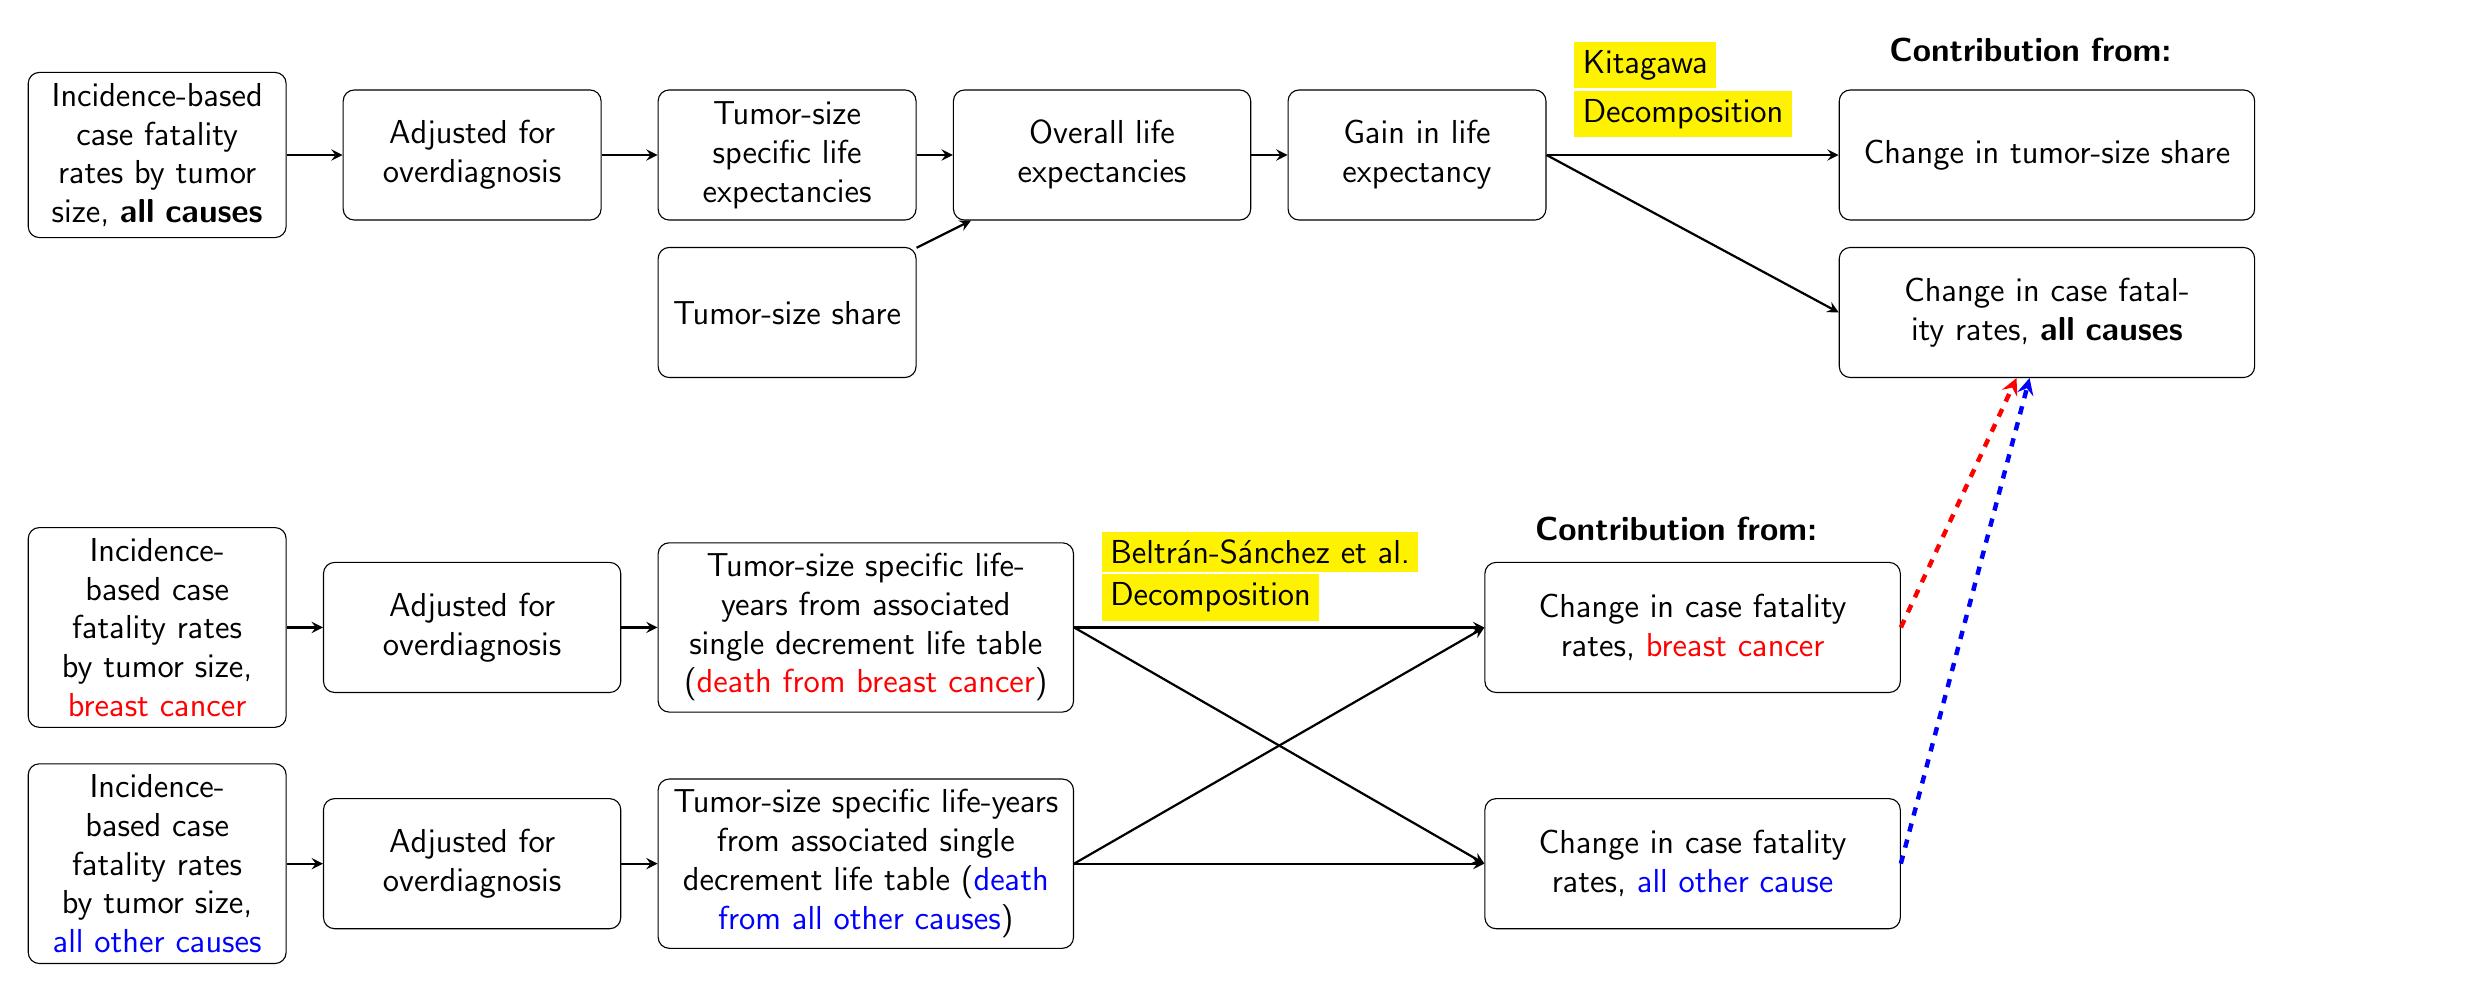
\begin{tikzpicture}[node distance = 4cm, auto]
  \large \node [block,text width=3cm] (n1) {Incidence-based case fatality rates by tumor size, \textbf{all causes}};
  \large \node [block, text width=3cm, right of=n1](n2){Adjusted for overdiagnosis};
 \large \node [block, text width=3cm, right of=n2](n4){Tumor-size specific life expectancies};
  \large \node [block, text width=3cm, below of=n4, yshift=2cm](n4a){Tumor-size share};
  \large \node [block, text width=3.5cm, right of=n4](n5){Overall life expectancies};
  \large \node [block, text width=3cm, right of=n5](n6){Gain in life expectancy};
  \large \node [block, text width=5cm, right
  of=n6,xshift=4cm](n7){Change in tumor-size share};
  \large \node [block, text width=5cm, yshift=2cm, below
  of=n7](n8){Change in case fatality rates, \textbf{all causes}};


 \path[->,thick] (n1) edge (n2);
 \path[->,thick] (n2) edge (n4);
 \path[->,thick] (n4) edge (n5);
 \path[->,thick] (n4a) edge (n5);
 \path[->,thick] (n5) edge (n6);
 \path[->,thick] (n6) edge (n7);
 \path[->,thick] (n6.east) edge (n8.west);

 \node [text width=7cm,xshift=1.5cm,yshift=0.5cm] (ctf) at (n7.north) {\textbf{Contribution from:}};
 \node [text width=7cm,xshift=5.5cm] (kitigawa) at (n6.north) {\hlight{Kitagawa} \\\hlight{Decomposition}};
 
 \large \node [block,text width=3cm,below of=n1,yshift=-2cm] (n9)
 {Incidence-based case fatality rates by tumor size, \tcr{breast cancer}};
 \large \node [block,text width=3cm,yshift=1cm,below of=n9] (n10)
 {Incidence-based case fatality rates by tumor size, \tcb{all other causes}};
  
  \large \node [block, text width=3.5cm, right
  of=n9](n11){Adjusted for overdiagnosis};
  \large \node [block, text width=3.5cm, right
  of=n10](n12){Adjusted for overdiagnosis};

 
\large \node [block, text width=5cm, xshift=1cm,right of=n11](n15){Tumor-size specific life-years from associated
  single decrement life table (\tcr{death from
  breast cancer})};
\large \node [block, text width=5cm, xshift=1cm,right of=n12](n16){Tumor-size specific life-years from associated
  single decrement life table  (\tcb{death from
  all other causes})};

 \large \node [block, text width=5cm, right of=n15,
 xshift=6.5cm](n17){Change in case fatality rates,
   \tcr{breast cancer}};
 \large \node [block, text width=5cm, right of=n16,
 xshift=6.5cm](n18){Change in case fatality rates,
   \tcb{all other cause}};

  \node [text width=7cm,xshift=1.5cm,yshift=1.25cm] (ctf) at (n17) {\textbf{Contribution from:}};
\node [text width=7cm,xshift=-4cm,yshift=0.65cm] (hbs) at (n17) {\hlight{Beltr\'{a}n-S\'{a}nchez et al.}\\ \hlight{Decomposition}};

 \path[->,thick] (n9) edge (n11);
 \path[->,thick] (n11) edge (n15);
 \path[->,thick] (n15) edge (n17);
 \path[->,thick] (n15.east) edge (n18.west);

 \path[->,thick] (n10) edge (n12);
 \path[->,thick] (n12) edge (n16);
 \path[->,thick] (n16) edge (n18);
\path[->,thick] (n16.east) edge (n17.west);
 
 \path[->,ultra thick,dashed,red] (n17.east) edge (n8); 
 \path[->,ultra thick,dashed,blue] (n18.east) edge (n8); 
\end{tikzpicture}
\end{document}